
\subsubsection{Insight Maker}
Insight Maker is a powerful online tool used to model and simulate utilizing different approaches, such as System Dynamics, Agent-Based Modeling and imperative programming. Insight Maker allows to construct a graphical model interface to forecast the system response \cite{FortmannRoe}. The implemented Insight Maker SD model is depicted in Figure \ref{fig:SD_IM}.

\begin{figure}[!h]
  \centering
%  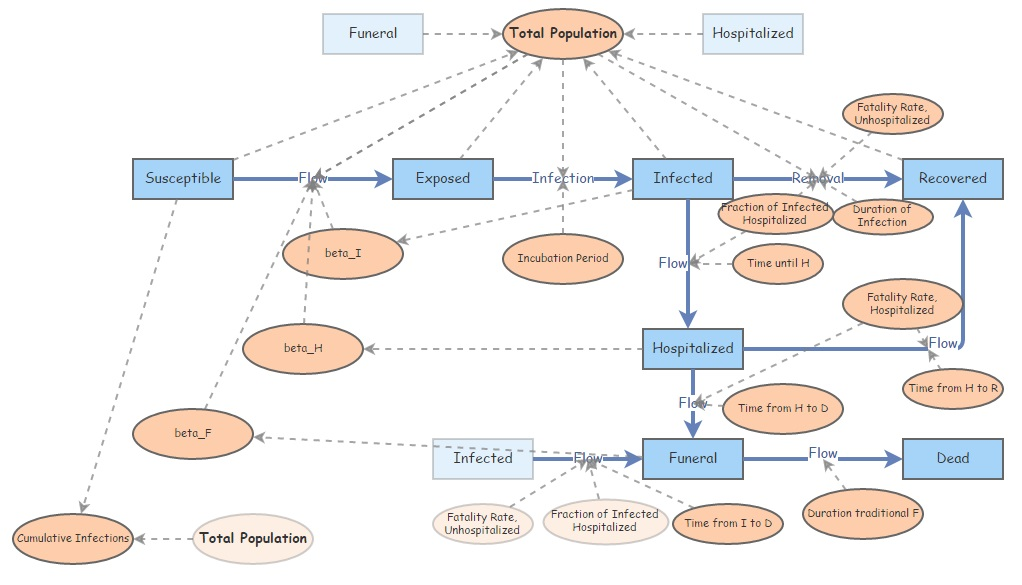
\includegraphics[width=0.7\textwidth]{SD_IM}
  \caption{ \bf Compartment model of the system dynamics implemented on Insight Maker}
\label{fig:SD_IM} 
\end{figure}

Based on the compartmental model and parameters published by Rivers et al.\cite{Rivers2014} in October 2014, it was modeled a similar approach in Insight Maker.  This particular model, divides the population into six different compartments; the Susceptible persons (S) could turn into Exposed (E), if they were in contact with an infections individual, initiating a transition to the Infectious (I) state after the incubation period of the disease, subsequently, acquiring the capacity of infecting others. A percentage of the I class individuals may be Hospitalized (H). There are two possible outcomes for the untreated individuals in I and the treated patients in H, individuals may die, with a probability of infecting other people during the resultant Funeral (F), before the virus is removed from the individual (R), or the patients may recover, at this stage, it can be considered equivalently removed. However, for the present study was considered seven compartments in order to distinguish between the recovered (R) patients and the deceased (D) individuals. Figure ~\ref{fig:compartment} depicts the implemented compartment model. \\

A normalized population fraction was simulated. The compartment S was initialized with a value of 999.999/1.000.000, and the compartment I with 1/1.000.000, meaning that there is a infected individual per every million of habitants, the rest of the compartments were set as 0. The flow between the compartments is specified in Figure \ref{fig:compartment} and all the other parameters were initialized as shown in Table \ref{tab:parameters}.  As mention in Section CALIBRATION SECTION, the parameters were calibrated in two stages, before and after the international intervention. The change on these parameters according with the time frame, was also implemented in Insight Maker.\\

\begin{figure}[h!]
  \centering
%  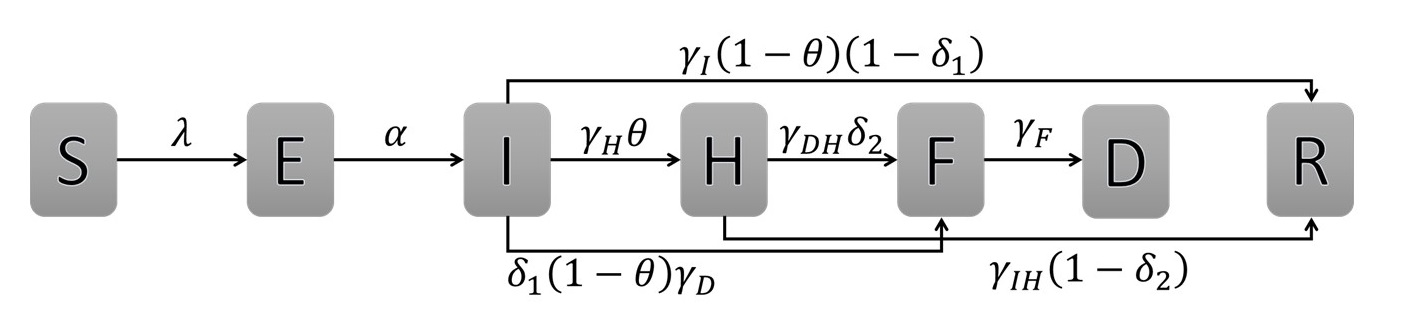
\includegraphics[width=0.7\textwidth]{compartment}
  \caption{Compartment Model of the Ebola Epidemic in Liberia and Sierra Leone \newline  Being S: Susceptible, E: Exposed, I: Infectious, H: Hospitalized, F: Funeral,  R: Recovered and D: Dead. All the possible flows are specified by the arrows and the parameters that direct them. Note that $\lambda = \beta_{I}I+\beta_{H}H+\beta_{F}F $, being a combination of all the $\beta$ transmission terms shown in Table~\ref{tab:parameters}} 
\label{fig:compartment} 
\end{figure}

 
The governing equations of the system described above are the following:
\begin{align*} 
\frac{dS}{dt} &= - \frac{\beta_{I}SI+\beta_{H}SH+\beta_{F}SF}{N}\\
\frac{dE}{dt} &=  \frac{\beta_{I}SI+\beta_{H}SH+\beta_{F}SF}{N}-\alpha E\\
\frac{dI}{dt} &=  \alpha E - [\gamma_{H}\theta + \gamma_{I}(1-\theta)(1-\delta_{1})+\gamma_{D}(1-\theta)\delta_{1}]I\\
\frac{dH}{dt} &= \gamma_{H}\theta I - [\gamma_{DH}\delta_{2}+\gamma_{IH}(1-\delta_{2})]H\\
\frac{dF}{dt} &= \gamma_{D}(1-\theta) \delta_{1} I + \gamma_{DH}\delta_{2} H-\gamma_{F} F\\
\frac{dR}{dt} &= \gamma_{I}(1-\theta)(1- \delta_{1}) I + \gamma_{IH}(1-\delta_{2}) H-\gamma_{F} F
\end{align*}
where each of the parameters are defined on Table \ref{tab:parameters}


\begin{table}[ht]
\caption{Model Parameters for Ebola Epidemic in Liberia Before  and After the International Intervention} % title of Table
\centering % used for centering table
\begin{tabular}{c c c } 
\hline\hline %inserts double horizontal lines
Parameter & Liberia Before Intervention  & Liberia After Intervention \\ [0.5ex] 
 & (Mar/14 to Sept/14) &  (Sept/14 to Jul/15) \\ [0.5ex] % inserts table
% inserts table
%heading
\hline % inserts single horizontal line
Contact Rate, Community  ($\beta_{I}$) & 0.148 & 0.0446  \\ 
Contact Rate, Hospital  ($\beta_{H}$) & 0.235 & 0.0877  \\
Contact Rate, Funeral  ($\beta_{F}$) & 0.465 & 0.283 \\
Incubation Period (${1}/{\alpha}$) & 11 days & 11 days  \\
Time until Hospitalization (${1}/{\gamma_{H}}$) & 4.49 days & 4.63 days  \\
Time from Hospitalization to Death (${1}/{\gamma_{DH}}$) & 3.51 days & 3.51 days  \\ 
Duration of Traditional Funeral (${1}/{\gamma_{F}}$) & 2.00 days & 2.00 days  \\
Duration of Infection (${1}/{\gamma_{I}}$) & 10.00 days & 10.00 days  \\
Time from Infection to Death (${1}/{\gamma_{D}}$) & 8.00 days & 8.00 days  \\
Time from Hospitalization to Recovery (${1}/{\gamma_{IH}}$) & 5.51 days & 5.51 days  \\
Probability a Case is Hospitalized ($\theta$) & 0.248 & 0.233 \\
Case Fatality Rate, Unhospitalized ($\delta_{1}$) & 0.500  & 0.500  \\
Case Fatality Rate, Hospitalized ($\delta_{2}$) & 0.500 & 0.500 \\ [1ex] 
\hline 
\end{tabular}
\label{tab:parameters}
\end{table}

%\begin{figure}
%\begin{tikzpicture}[->,>=stealth',shorten >=1pt,auto,node distance=3cm,
%  thick,main node/.style={circle,fill=blue!20,draw,font=\sffamily\Large\bfseries}]
%
%  \node[main node] (1) {S};
%  \node[main node] (2) [right of=1] {E};
%  \node[main node] (3) [right of=2] {I};
%  \node[main node] (4) [right of=3] {R};
%    \node[main node] (5) [below left of=3] {D};
%      \node[main node] (6) [below right of=3] {F};
%        \node[main node] (7) [right of=6] {H};
%
%  \path[every node/.style={font=\sffamily\small}]
%    (1)
%        edge node {$f_{SE}$} (2)
% 
%    (2) edge node {$f_{EI}$} (3)
%        
%    (3) 
%       edge node {$f_{IR}$} (4)
%       edge node[left] {$f_{IF}$} (6)
%       edge node {$f_{IH}$} (7)
%  
%    (4)
%       
%(6) edge node{$f_{FD}$} (5) 
%
%(7) edge node[right]{$f_{HR}$} (4) 
%
%  (7) edge node{$f_{HF}$} (6)      
%
%        ;
%        
%\end{tikzpicture}
%\caption{Model}
%\label{SM}
%\end{figure}